\section{Auswertung}
\subsection{Bestimmung der Molwärme}
Da sich die Bestimmung der Molwärme bei konstanten Volumen experimentell schwierig gestaltet, wird sattdessen die Molwärme bei konstanten Druck über die Zusammenhänge
\begin{align}
    E = U \cdot I \symup{\Delta} t \\
    c_p = \frac{M}{m} \cdot \frac{E}{\symup{\Delta T}}
\end{align}
\begin{center}
    \tiny{($E \hat{=} \text{Energie}$, $U \hat{=} \text{Spannung}$, $I \hat{=} \text{Stromstärke}$, $t \hat{=} \text{Zeit}$, $T \hat{=} \text{Energie}$, $m \hat{=} \text{Masse}$, $M \hat{=} \text{Molare Masse}$)}
\end{center}
bestimmt. Die zur Berechnung benötigten Daten befinden sich in Tabelle \ref{tab:cp}. Von dem gemessenen Widerstand der Probe lässt sich über den Zusammenhang
\begin{equation}
    T=\SI{0.00134}{\kelvin\per\ohm\squared}R^2+\SI{2.296}{\kelvin\per\ohm}R+\SI{30.13}{\kelvin}
\end{equation}
auf die Temperatur $T$ schließen.
\begin{longtable}{ c c c c c c c } 
   \caption{Aufgenommene Messwerte zur Bestimmung der Wärmekapazität. Die Indizes $p$ und $z$ dienen zur Unterschiedung zwischen der Probe $p$ und dem Zylinder $z$.} 
   \label{tab:cp} \\
    \toprule
 {$t\:/\: \mathrm{s}$} & {$R_p\:/\: \Omega$} & {$R_z\:/\: \Omega$} & {$U\:/\: \mathrm{V}$} & {$I_p\:/\: \mathrm{A}$} & {$I_z\:/\: \mathrm{A}$} & {$C_p\:/\: \mathrm{J/(kg \cdot K)}$} \\ 
    \midrule 
    \endfirsthead
    \caption{ (Fortsetzung)} \\
    \toprule
    {$t\:/\: \mathrm{s}$} & {$R_p\:/\: \mathrm{\Omega}$} & {$R_z\:/\: \mathrm{\Omega}$} & {$U\:/\: \mathrm{V}$} & {$I_p\:/\: \mathrm{A}$} & {$I_z\:/\: \mathrm{A}$} & {$C_p\:/\: \mathrm{J/(kg \cdot K)}$} \\ 
    \midrule
  \endhead
    \midrule
  \endfoot
    \bottomrule
  \endlastfoot 
     150 &  21,8 &  22,0 & 16,73 & 159,8 & 4,0 &  0.9 \pm 0.0 \\ 
     300 &  24,0 &  23,3 & 16,76 & 159,9 & 4,0 & 14.4 \pm 0.9 \\ 
     450 &  26,0 &  25,0 & 16,83 & 160,5 & 4,4 & 15.9 \pm 1.1 \\ 
     600 &  27,9 &  27,0 & 16,88 & 160,8 & 4,4 & 16.8 \pm 1.3 \\ 
     750 &  29,7 &  29,0 & 16,91 & 161,0 & 4,8 & 17.8 \pm 1.4 \\ 
     900 &  31,6 &  31,3 & 16,94 & 161,2 & 4,8 & 16.8 \pm 1.3 \\ 
    1050 &  33,4 &  33,6 & 16,97 & 161,4 & 4,6 & 17.8 \pm 1.4 \\ 
    1200 &  35,2 &  35,8 & 16,99 & 161,5 & 4,6 & 17.8 \pm 1.4 \\ 
    1350 &  37,0 &  38,0 & 17,01 & 161,6 & 4,6 & 17.8 \pm 1.4 \\ 
    1500 &  38,8 &  40,2 & 17,03 & 161,7 & 4,6 & 17.8 \pm 1.4 \\ 
    1650 &  40,6 &  42,5 & 17,04 & 161,8 & 4,4 & 17.8 \pm 1.4 \\ 
    1800 &  42,5 &  44,7 & 17,06 & 161,8 & 4,3 & 16.8 \pm 1.3 \\ 
    1950 &  44,3 &  46,7 & 17,07 & 161,9 & 4,0 & 17.7 \pm 1.4 \\ 
    2100 &  46,0 &  48,5 & 17,09 & 161,9 & 4,0 & 18.8 \pm 1.6 \\ 
    2250 &  47,9 &  50,3 & 17,10 & 162,0 & 3,9 & 16.8 \pm 1.2 \\ 
    2400 &  49,6 &  51,8 & 17,11 & 162,1 & 3,9 & 18.7 \pm 1.6 \\ 
    2550 &  51,3 &  53,7 & 17,12 & 162,2 & 4,0 & 18.7 \pm 1.6 \\ 
    2700 &  52,9 &  54,9 & 17,13 & 162,2 & 3,8 & 19.9 \pm 1.8 \\ 
    2850 &  54,5 &  56,5 & 17,13 & 162,2 & 3,8 & 19.8 \pm 1.8 \\ 
    3000 &  56,1 &  57,7 & 17,14 & 162,3 & 3,8 & 19.8 \pm 1.8 \\ 
    3150 &  57,7 &  58,8 & 17,15 & 162,3 & 3,8 & 19.8 \pm 1.8 \\ 
    3300 &  59,2 &  59,9 & 17,15 & 162,3 & 3,8 & 21.1 \pm 2.0 \\ 
    3450 &  60,6 &  60,9 & 17,16 & 162,4 & 3,8 & 22.6 \pm 2.3 \\ 
    3600 &  62,0 &  61,8 & 17,16 & 162,4 & 3,9 & 22.5 \pm 2.3 \\ 
    3750 &  63,4 &  62,9 & 17,17 & 162,4 & 3,9 & 22.5 \pm 2.3 \\ 
    3900 &  64,8 &  64,3 & 17,17 & 162,5 & 4,0 & 22.5 \pm 2.3 \\ 
    4050 &  66,1 &  65,7 & 17,17 & 162,5 & 4,0 & 24.2 \pm 2.6 \\ 
    4200 &  67,5 &  67,0 & 17,17 & 162,5 & 4,1 & 22.4 \pm 2.3 \\ 
    4350 &  68,8 &  68,8 & 17,18 & 162,5 & 4,2 & 24.1 \pm 2.6 \\ 
    4500 &  70,2 &  70,5 & 17,18 & 162,6 & 4,2 & 22.4 \pm 2.3 \\ 
    4650 &  71,5 &  72,5 & 17,18 & 162,6 & 4,0 & 24.1 \pm 2.6 \\ 
    4800 &  73,0 &  74,3 & 17,19 & 162,6 & 3,8 & 20.9 \pm 2.0 \\ 
    4950 &  74,4 &  76,0 & 17,19 & 162,6 & 3,8 & 22.3 \pm 2.3 \\ 
    5100 &  75,8 &  77,3 & 17,19 & 162,7 & 3,6 & 22.3 \pm 2.3 \\ 
    5250 &  77,2 &  78,5 & 17,19 & 162,7 & 3,6 & 22.3 \pm 2.2 \\ 
    5400 &  78,6 &  79,5 & 17,20 & 162,7 & 3,6 & 22.2 \pm 2.2 \\ 
    5700 &  80,0 &  80,5 & 17,19 & 162,7 & 3,6 & 44.0 \pm 4.0 \\ 
    6000 &  82,7 &  82,1 & 17,20 & 162,7 & 3,6 & 23.0 \pm 1.2 \\ 
    6300 &  85,0 &  83,7 & 17,20 & 162,8 & 3,6 & 26.9 \pm 1.7 \\ 
    6600 &  87,1 &  85,6 & 17,20 & 162,8 & 3,8 & 29.4 \pm 2.0 \\ 
    6900 &  89,3 &  88,4 & 17,20 & 162,7 & 4,0 & 28.0 \pm 1.8 \\ 
    7200 &  91,7 &  91,5 & 17,20 & 162,9 & 4,0 & 25.6 \pm 1.5 \\ 
    7500 &  94,3 &  94,8 & 17,20 & 163,0 & 4,0 & 23.6 \pm 1.3 \\ 
    7800 &  97,0 &  97,3 & 17,20 & 163,0 & 3,8 & 22.7 \pm 1.2 \\ 
    8100 &  99,4 &  99,2 & 17,19 & 163,0 & 3,8 & 25.4 \pm 1.5 \\ 
    8400 & 101,9 & 101,2 & 17,19 & 163,0 & 3,8 & 24.3 \pm 1.4 \\ 
    8700 & 104,2 & 103,9 & 17,19 & 162,9 & 4,0 & 26.4 \pm 1.6 \\ 
    9000 & 106,6 & 106,6 & 17,19 & 162,9 & 4,0 & 25.2 \pm 1.5 \\ 
    9300 & 109,1 & 109,2 & 17,19 & 162,9 & 4,0 & 24.2 \pm 1.4 \\ 
    9600 & 111,5 & 111,6 & 17,18 & 163,0 & 4,0 & 25.1 \pm 1.5 \\ 
\end{longtable}
In Tabelle \ref{tab:alpha} befinden sich lineare Ausdehnungskoeffizienten zu gegebenen Temperaturen. Um den linearen Ausdehnungskoeffizienten genauer an die gemessene Temperatur anzugleichen, wurde eine Ausgleichsrechnung der Form
\begin{equation}
    \alpha = \frac{m}{T}+b
\end{equation}
\begin{center}
    \tiny{($m, b \hat{=} \text{Fitparameter}$)}
\end{center}
durchgeführt. Der Fit befindet sich in Abbildung \ref{fig:alpha}.
\begin{table}[H] 
   \centering 
   \caption{Die angegebenen Werte für den linearen Ausdehnungskoeffizienten} 
   \label{tab:alpha} 
   \begin{tabular} { c c } 
 \toprule 
 {$T\:/\: \mathrm{K}$} & {$\alpha\:/\: \mathrm{\mu K^{-1}}$} \\ 
    \midrule 
    70 & 7,00 \\ 
    80 & 8,50 \\ 
    90 & 9,75 \\ 
    100 & 10,70 \\ 
    110 & 11,50 \\ 
    120 & 12,10 \\ 
    130 & 12,65 \\ 
    140 & 13,15 \\ 
    150 & 13,60 \\ 
    160 & 13,90 \\ 
    170 & 14,25 \\ 
    180 & 14,50 \\ 
    190 & 14,75 \\ 
    200 & 14,95 \\ 
    210 & 15,20 \\ 
    220 & 15,40 \\ 
    230 & 15,60 \\ 
    240 & 15,75 \\ 
    250 & 15,90 \\ 
    260 & 16,10 \\ 
    270 & 16,25 \\ 
    280 & 16,35 \\ 
    290 & 16,50 \\ 
    300 & 16,65 \\ 
    \bottomrule 
  \end{tabular}
\end{table}
\begin{figure}[H]
    \centering
    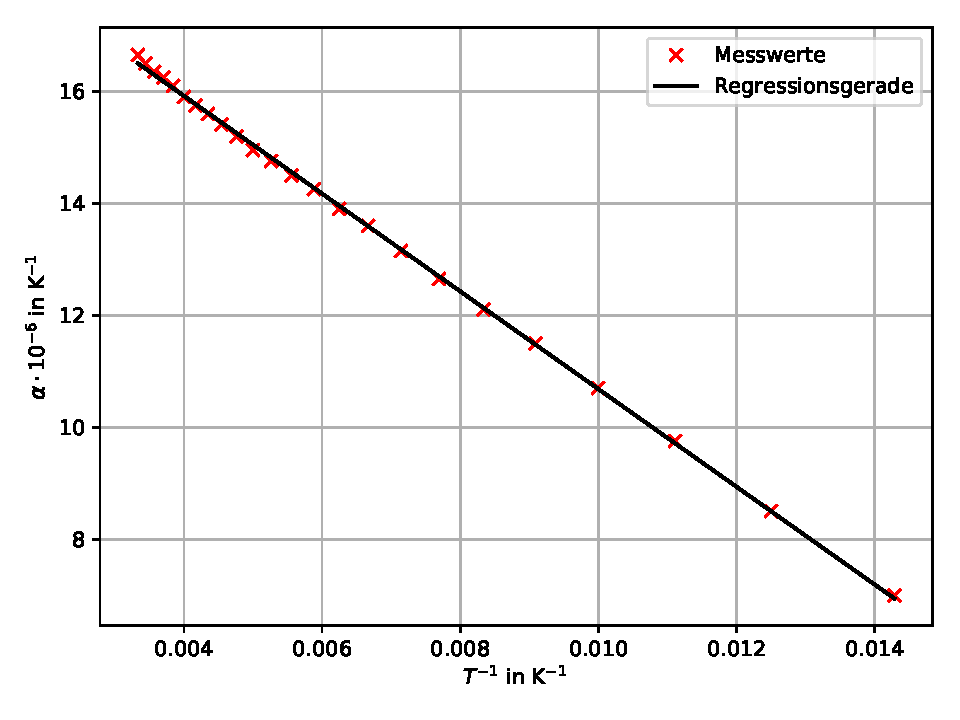
\includegraphics[ width= 0.8\textwidth]{data/plots/plot_alpha.pdf}
    \caption{Linearer Ausdehnungskoeffizient $\alpha$ von Kupfer aufgetragen gegen die inverse Temperatur $T$.}
    \label{fig:alpha}
\end{figure}
Für die Fitparameter folgt
\begin{align}
    m &=  -873 \pm 4 \\
    b &=  19.411 \pm 0.029 \si{\kelvin} .
\end{align}

In Abbildung \ref{fig:cvcp} sind abschließend die berechneten Werte für $C_V$ und $C_p$ gegen die Temperatur aufgetragen. Dabei berechnet sich $C_V$ für ein gegebenes $C_p$ über die Gleichung
\begin{equation}
    C_V = C_p - 9 \alpha^2 \kappa V_0 T
\end{equation}
\begin{center}
    \tiny{($\kappa \hat{=} \text{Kompressionsmodul} $, $V_0 \hat{=} \text{Molvolumen} $ )}
\end{center}
\begin{figure}[H]
    \centering
    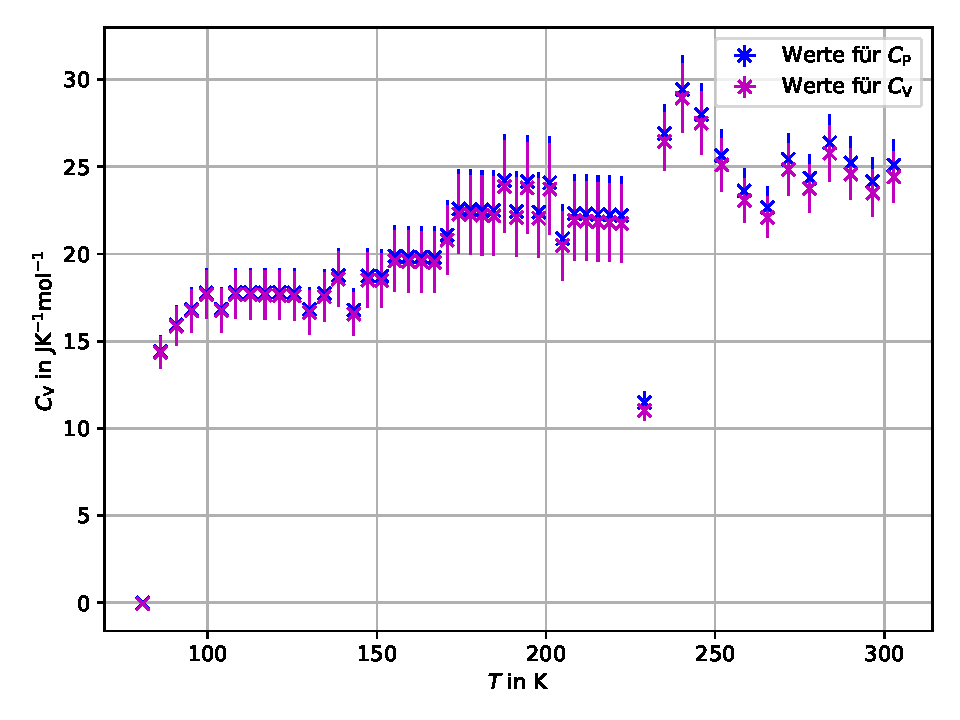
\includegraphics[width=0.8\textwidth]{data/plots/plot_Cv.pdf}
    \caption{Die Molwärmen in Abhängigkeit von der Temperatur.}
    \label{fig:cvcp}
\end{figure}

\subsection{Bestimmung der Debeye-Temperatur}
Mithilfe Gleichung \ref{eqn:debeye} kann die Debeye-temperatur für ein gegebenes Material bestimmt werden.
Durch die Forderung
\begin{equation}
	\int_0^{\omega_D} Z(\omega)d\omega = \frac{L^3}{2\pi^2}\omega^2\left(\frac{1}{v_\text{l}^3}+\frac{2}{v_{\text{t}}^3}\right)d\omega. \overset{!}{=} = 3 N_L
	\label{eqn:z}
\end{equation}
\begin{center}
    \tiny{($N_L \hat{=} \text{Loschmditsche Zahl}$, $L \hat{=} \text{Länge der Probe}$, $v_t \hat{=} \text{transversale Schallgeschwindigkeit}$, $v_l \hat{=} \text{longitudinale Schallgeschwindigkeit}$)}
\end{center}
folgt
\begin{equation}
    \left[\frac{18\pi^2N_L}{L^3}\left(\frac{1}{v_\text{l}^3}+\frac{2}{v_\text{tr}^3}\right)^{-1} \right]^{\frac{1}{3}} = \omega_D.
\end{equation}
Da die Länge der Probe nicht bekannt, muss dieser Faktor eliminiert werden. Mithilfe der Gleichungen
\begin{align}
    L^3 &= V = \frac{m}{\rho} \\
    N_L &= N_A \cdot \frac{m}{M}
\end{align}
\begin{center}
    \tiny{($N_A \hat{=} \text{Avogado-konstante}$)}
\end{center}
folgt mit $m = \SI{342}{\gram} $, $v_l = \SI{4,7}{\kilo \meter \per \second} $ und $v_t = \SI{2,26}{\kilo \meter \per \second}$ :
\begin{equation}
    \theta_{\mathrm{D},2}=\frac{\hbar}{k_{\mathrm{B}}}\sqrt[3]{\frac{18\pi^2N_A\rho}{M}\left(v_{\mathrm{long}}^{-3}+2v_{\mathrm{trans}}^{-3}\right)^{-1}}=\SI{332}{\kelvin}.
\end{equation}

Experimentell wird die Debeye-Temperatur $\sigma_D$ mithilfe der in Abbildung \ref{fig:deb} zu sehenden Tabelle bestimmt. Für ein gegebenes $C_V$ kann dort der entsprechende Wert $\frac{\theta_D}{T}$ abgelesen werden. Über den Zusammenhang
\begin{equation}
    \theta_D = \frac{\theta_D}{T} \cdot T
    \label{eqn:theta}
\end{equation}
kann damit auf die Debeye-Temperatur geschlossen werden.
Wie in Abbildung \ref{fig:cvcp} zu sehen ist, ist der Verlauf zwischen $\SI{84}{\kelvin}$ und $\SI{170}{\kelvin}$ annähernd linear, weshalb in diesem Bereich die Debeye-Temperatur bestimmt wird.
Mit Gleichung \eqref{eqn:theta}
ergeben sich die in Abbildung \ref{fig:deb} zu sehenden Debeye-Temperaturen. 
Eine Mittelung über alle Werte ergibt:
\begin{equation}
    \theta_{D_{exp}} = 346 \pm 11 \si{\kelvin}.
\end{equation}
\begin{figure}
    \centering
    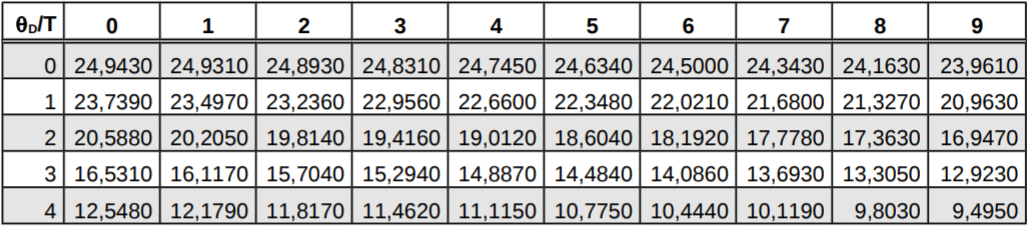
\includegraphics[width=0.9\textwidth]{content/images/table1.png}
    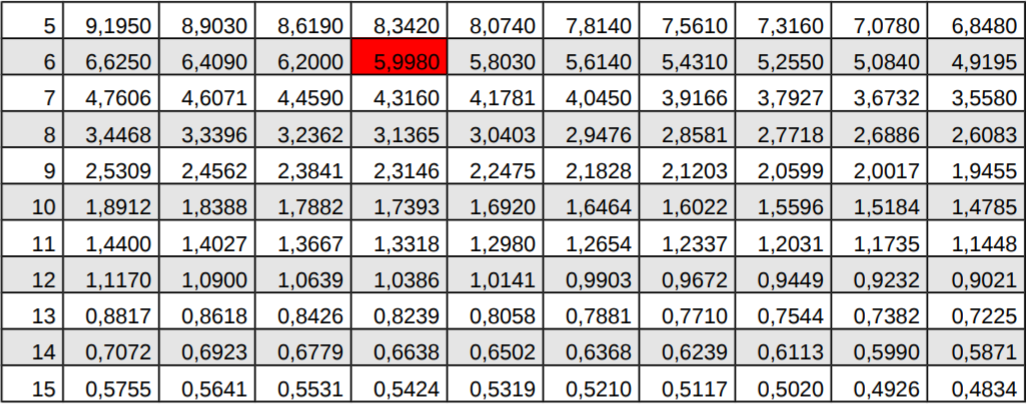
\includegraphics[width=0.9\textwidth]{content/images/table2.png}
    \caption{Zahlenwerte der Debye-Funktion \cite{anleitung}.}
    \label{fig:deb}
\end{figure}
